% Options for packages loaded elsewhere
\PassOptionsToPackage{unicode}{hyperref}
\PassOptionsToPackage{hyphens}{url}
\PassOptionsToPackage{dvipsnames,svgnames,x11names}{xcolor}
%
\documentclass[
  letterpaper,
  DIV=11,
  numbers=noendperiod]{scrartcl}

\usepackage{amsmath,amssymb}
\usepackage{iftex}
\ifPDFTeX
  \usepackage[T1]{fontenc}
  \usepackage[utf8]{inputenc}
  \usepackage{textcomp} % provide euro and other symbols
\else % if luatex or xetex
  \usepackage{unicode-math}
  \defaultfontfeatures{Scale=MatchLowercase}
  \defaultfontfeatures[\rmfamily]{Ligatures=TeX,Scale=1}
\fi
\usepackage{lmodern}
\ifPDFTeX\else  
    % xetex/luatex font selection
\fi
% Use upquote if available, for straight quotes in verbatim environments
\IfFileExists{upquote.sty}{\usepackage{upquote}}{}
\IfFileExists{microtype.sty}{% use microtype if available
  \usepackage[]{microtype}
  \UseMicrotypeSet[protrusion]{basicmath} % disable protrusion for tt fonts
}{}
\makeatletter
\@ifundefined{KOMAClassName}{% if non-KOMA class
  \IfFileExists{parskip.sty}{%
    \usepackage{parskip}
  }{% else
    \setlength{\parindent}{0pt}
    \setlength{\parskip}{6pt plus 2pt minus 1pt}}
}{% if KOMA class
  \KOMAoptions{parskip=half}}
\makeatother
\usepackage{xcolor}
\setlength{\emergencystretch}{3em} % prevent overfull lines
\setcounter{secnumdepth}{-\maxdimen} % remove section numbering
% Make \paragraph and \subparagraph free-standing
\ifx\paragraph\undefined\else
  \let\oldparagraph\paragraph
  \renewcommand{\paragraph}[1]{\oldparagraph{#1}\mbox{}}
\fi
\ifx\subparagraph\undefined\else
  \let\oldsubparagraph\subparagraph
  \renewcommand{\subparagraph}[1]{\oldsubparagraph{#1}\mbox{}}
\fi

\usepackage{color}
\usepackage{fancyvrb}
\newcommand{\VerbBar}{|}
\newcommand{\VERB}{\Verb[commandchars=\\\{\}]}
\DefineVerbatimEnvironment{Highlighting}{Verbatim}{commandchars=\\\{\}}
% Add ',fontsize=\small' for more characters per line
\usepackage{framed}
\definecolor{shadecolor}{RGB}{241,243,245}
\newenvironment{Shaded}{\begin{snugshade}}{\end{snugshade}}
\newcommand{\AlertTok}[1]{\textcolor[rgb]{0.68,0.00,0.00}{#1}}
\newcommand{\AnnotationTok}[1]{\textcolor[rgb]{0.37,0.37,0.37}{#1}}
\newcommand{\AttributeTok}[1]{\textcolor[rgb]{0.40,0.45,0.13}{#1}}
\newcommand{\BaseNTok}[1]{\textcolor[rgb]{0.68,0.00,0.00}{#1}}
\newcommand{\BuiltInTok}[1]{\textcolor[rgb]{0.00,0.23,0.31}{#1}}
\newcommand{\CharTok}[1]{\textcolor[rgb]{0.13,0.47,0.30}{#1}}
\newcommand{\CommentTok}[1]{\textcolor[rgb]{0.37,0.37,0.37}{#1}}
\newcommand{\CommentVarTok}[1]{\textcolor[rgb]{0.37,0.37,0.37}{\textit{#1}}}
\newcommand{\ConstantTok}[1]{\textcolor[rgb]{0.56,0.35,0.01}{#1}}
\newcommand{\ControlFlowTok}[1]{\textcolor[rgb]{0.00,0.23,0.31}{#1}}
\newcommand{\DataTypeTok}[1]{\textcolor[rgb]{0.68,0.00,0.00}{#1}}
\newcommand{\DecValTok}[1]{\textcolor[rgb]{0.68,0.00,0.00}{#1}}
\newcommand{\DocumentationTok}[1]{\textcolor[rgb]{0.37,0.37,0.37}{\textit{#1}}}
\newcommand{\ErrorTok}[1]{\textcolor[rgb]{0.68,0.00,0.00}{#1}}
\newcommand{\ExtensionTok}[1]{\textcolor[rgb]{0.00,0.23,0.31}{#1}}
\newcommand{\FloatTok}[1]{\textcolor[rgb]{0.68,0.00,0.00}{#1}}
\newcommand{\FunctionTok}[1]{\textcolor[rgb]{0.28,0.35,0.67}{#1}}
\newcommand{\ImportTok}[1]{\textcolor[rgb]{0.00,0.46,0.62}{#1}}
\newcommand{\InformationTok}[1]{\textcolor[rgb]{0.37,0.37,0.37}{#1}}
\newcommand{\KeywordTok}[1]{\textcolor[rgb]{0.00,0.23,0.31}{#1}}
\newcommand{\NormalTok}[1]{\textcolor[rgb]{0.00,0.23,0.31}{#1}}
\newcommand{\OperatorTok}[1]{\textcolor[rgb]{0.37,0.37,0.37}{#1}}
\newcommand{\OtherTok}[1]{\textcolor[rgb]{0.00,0.23,0.31}{#1}}
\newcommand{\PreprocessorTok}[1]{\textcolor[rgb]{0.68,0.00,0.00}{#1}}
\newcommand{\RegionMarkerTok}[1]{\textcolor[rgb]{0.00,0.23,0.31}{#1}}
\newcommand{\SpecialCharTok}[1]{\textcolor[rgb]{0.37,0.37,0.37}{#1}}
\newcommand{\SpecialStringTok}[1]{\textcolor[rgb]{0.13,0.47,0.30}{#1}}
\newcommand{\StringTok}[1]{\textcolor[rgb]{0.13,0.47,0.30}{#1}}
\newcommand{\VariableTok}[1]{\textcolor[rgb]{0.07,0.07,0.07}{#1}}
\newcommand{\VerbatimStringTok}[1]{\textcolor[rgb]{0.13,0.47,0.30}{#1}}
\newcommand{\WarningTok}[1]{\textcolor[rgb]{0.37,0.37,0.37}{\textit{#1}}}

\providecommand{\tightlist}{%
  \setlength{\itemsep}{0pt}\setlength{\parskip}{0pt}}\usepackage{longtable,booktabs,array}
\usepackage{calc} % for calculating minipage widths
% Correct order of tables after \paragraph or \subparagraph
\usepackage{etoolbox}
\makeatletter
\patchcmd\longtable{\par}{\if@noskipsec\mbox{}\fi\par}{}{}
\makeatother
% Allow footnotes in longtable head/foot
\IfFileExists{footnotehyper.sty}{\usepackage{footnotehyper}}{\usepackage{footnote}}
\makesavenoteenv{longtable}
\usepackage{graphicx}
\makeatletter
\def\maxwidth{\ifdim\Gin@nat@width>\linewidth\linewidth\else\Gin@nat@width\fi}
\def\maxheight{\ifdim\Gin@nat@height>\textheight\textheight\else\Gin@nat@height\fi}
\makeatother
% Scale images if necessary, so that they will not overflow the page
% margins by default, and it is still possible to overwrite the defaults
% using explicit options in \includegraphics[width, height, ...]{}
\setkeys{Gin}{width=\maxwidth,height=\maxheight,keepaspectratio}
% Set default figure placement to htbp
\makeatletter
\def\fps@figure{htbp}
\makeatother

\KOMAoption{captions}{tableheading}
\makeatletter
\@ifpackageloaded{tcolorbox}{}{\usepackage[skins,breakable]{tcolorbox}}
\@ifpackageloaded{fontawesome5}{}{\usepackage{fontawesome5}}
\definecolor{quarto-callout-color}{HTML}{909090}
\definecolor{quarto-callout-note-color}{HTML}{0758E5}
\definecolor{quarto-callout-important-color}{HTML}{CC1914}
\definecolor{quarto-callout-warning-color}{HTML}{EB9113}
\definecolor{quarto-callout-tip-color}{HTML}{00A047}
\definecolor{quarto-callout-caution-color}{HTML}{FC5300}
\definecolor{quarto-callout-color-frame}{HTML}{acacac}
\definecolor{quarto-callout-note-color-frame}{HTML}{4582ec}
\definecolor{quarto-callout-important-color-frame}{HTML}{d9534f}
\definecolor{quarto-callout-warning-color-frame}{HTML}{f0ad4e}
\definecolor{quarto-callout-tip-color-frame}{HTML}{02b875}
\definecolor{quarto-callout-caution-color-frame}{HTML}{fd7e14}
\makeatother
\makeatletter
\makeatother
\makeatletter
\makeatother
\makeatletter
\@ifpackageloaded{caption}{}{\usepackage{caption}}
\AtBeginDocument{%
\ifdefined\contentsname
  \renewcommand*\contentsname{Table of contents}
\else
  \newcommand\contentsname{Table of contents}
\fi
\ifdefined\listfigurename
  \renewcommand*\listfigurename{List of Figures}
\else
  \newcommand\listfigurename{List of Figures}
\fi
\ifdefined\listtablename
  \renewcommand*\listtablename{List of Tables}
\else
  \newcommand\listtablename{List of Tables}
\fi
\ifdefined\figurename
  \renewcommand*\figurename{Figure}
\else
  \newcommand\figurename{Figure}
\fi
\ifdefined\tablename
  \renewcommand*\tablename{Table}
\else
  \newcommand\tablename{Table}
\fi
}
\@ifpackageloaded{float}{}{\usepackage{float}}
\floatstyle{ruled}
\@ifundefined{c@chapter}{\newfloat{codelisting}{h}{lop}}{\newfloat{codelisting}{h}{lop}[chapter]}
\floatname{codelisting}{Listing}
\newcommand*\listoflistings{\listof{codelisting}{List of Listings}}
\makeatother
\makeatletter
\@ifpackageloaded{caption}{}{\usepackage{caption}}
\@ifpackageloaded{subcaption}{}{\usepackage{subcaption}}
\makeatother
\makeatletter
\@ifpackageloaded{tcolorbox}{}{\usepackage[skins,breakable]{tcolorbox}}
\makeatother
\makeatletter
\@ifundefined{shadecolor}{\definecolor{shadecolor}{rgb}{.97, .97, .97}}
\makeatother
\makeatletter
\makeatother
\makeatletter
\makeatother
\ifLuaTeX
  \usepackage{selnolig}  % disable illegal ligatures
\fi
\IfFileExists{bookmark.sty}{\usepackage{bookmark}}{\usepackage{hyperref}}
\IfFileExists{xurl.sty}{\usepackage{xurl}}{} % add URL line breaks if available
\urlstyle{same} % disable monospaced font for URLs
\hypersetup{
  pdftitle={Webscraping Text},
  pdfauthor={Emily Malcolm-White},
  colorlinks=true,
  linkcolor={blue},
  filecolor={Maroon},
  citecolor={Blue},
  urlcolor={Blue},
  pdfcreator={LaTeX via pandoc}}

\title{Webscraping Text}
\author{Emily Malcolm-White}
\date{}

\begin{document}
\maketitle
\ifdefined\Shaded\renewenvironment{Shaded}{\begin{tcolorbox}[breakable, enhanced, boxrule=0pt, sharp corners, frame hidden, interior hidden, borderline west={3pt}{0pt}{shadecolor}]}{\end{tcolorbox}}\fi


\includegraphics[width=0.3\textwidth,height=\textheight]{118_P_webscraping_text_files/mediabag/logo.png}

\begin{Shaded}
\begin{Highlighting}[]
\CommentTok{\#LOAD PACKAGES }
\FunctionTok{library}\NormalTok{(tidyverse)}
\FunctionTok{library}\NormalTok{(rvest)}
\end{Highlighting}
\end{Shaded}

\hypertarget{webscraping-text}{%
\section{Webscraping Text}\label{webscraping-text}}

Let's look at the
\href{https://www.imdb.com/search/title/?title_type=feature\&year=2023-01-01,2023-07-31}{top
50 feature films in the first 7 months of 2023 listed on IMBD}

\begin{Shaded}
\begin{Highlighting}[]
\NormalTok{URL }\OtherTok{\textless{}{-}} \FunctionTok{read\_html}\NormalTok{(}\StringTok{"https://www.imdb.com/search/title/?title\_type=feature\&year=2023{-}01{-}01,2023{-}07{-}31"}\NormalTok{)}
\end{Highlighting}
\end{Shaded}

Notice that the data for all these films isn't housed inside a
\texttt{\textless{}table\textgreater{}} element!

\hypertarget{titles}{%
\subsection{Titles}\label{titles}}

For example, check out the first few lines of html code for Oppenheimer:

\begin{verbatim}
<h3 class="lister-item-header">
        <span class="lister-item-index unbold text-primary">1.</span>
    <a href="/title/tt15398776/?ref_=adv_li_tt"
>Oppenheimer</a>
    <span class="lister-item-year text-muted unbold">(2023)</span>
</h3>
\end{verbatim}

In this case, we want to look for the class \texttt{lister-item-header}
AND then pull the text inside the \texttt{\textless{}a\textgreater{}}
(link) tag.

\texttt{html\_elements(".lister-item-header\ a")}

\begin{tcolorbox}[enhanced jigsaw, arc=.35mm, left=2mm, colbacktitle=quarto-callout-tip-color!10!white, coltitle=black, leftrule=.75mm, rightrule=.15mm, opacitybacktitle=0.6, titlerule=0mm, colframe=quarto-callout-tip-color-frame, toptitle=1mm, breakable, bottomtitle=1mm, bottomrule=.15mm, opacityback=0, title=\textcolor{quarto-callout-tip-color}{\faLightbulb}\hspace{0.5em}{Tip}, toprule=.15mm, colback=white]

In this case, we want ALL titles so we used \texttt{html\_elements()}.
If we had only wanted the first title we would have used
\texttt{html\_element()}

\end{tcolorbox}

Scrape IMBD for the titles of the 50 most popular feature films in the
first 7 months of 2023.

\begin{Shaded}
\begin{Highlighting}[]
\CommentTok{\# title\_data \textless{}{-} URL \%\textgreater{}\%}
\CommentTok{\#   html\_elements(".lister{-}item{-}header a") \%\textgreater{}\%}
\CommentTok{\#   html\_text()}
\CommentTok{\# }
\CommentTok{\# title\_data}
\end{Highlighting}
\end{Shaded}

\hypertarget{runtime}{%
\subsection{Runtime}\label{runtime}}

Scrape IMBD for the runtime of the 50 most popular feature films so far
in 2023.

Check out the relevant HTML code for Oppenheimer:

\begin{verbatim}
    <p class="text-muted ">
            <span class="certificate">R</span>
                 <span class="ghost">|</span> 
                 <span class="runtime">180 min</span>
                 <span class="ghost">|</span> 
            <span class="genre">
Biography, Drama, History            </span>
    </p>
\end{verbatim}

In this case, we need to reference the class \texttt{text-muted} AND the
class \texttt{runtime}.

\begin{Shaded}
\begin{Highlighting}[]
\CommentTok{\# URL \%\textgreater{}\%}
\CommentTok{\#   html\_nodes(".text{-}muted .runtime") \%\textgreater{}\%}
\CommentTok{\#   html\_text() }
\end{Highlighting}
\end{Shaded}

Alternatively, we could have called class \texttt{text-muted} AND the
3rd span, but it's easier and likely more accurate to ask for the class
\texttt{runtime} in case \texttt{runtime} is missing for some reason.

Maybe we want to keep the \texttt{min} on the end, but it forces it into
being a stringr rather than a number which makes it difficult to sort or
filter.

\begin{Shaded}
\begin{Highlighting}[]
\FunctionTok{library}\NormalTok{(readr)}
\CommentTok{\# need this package for parse\_number()}
\end{Highlighting}
\end{Shaded}

\begin{figure}

{\centering 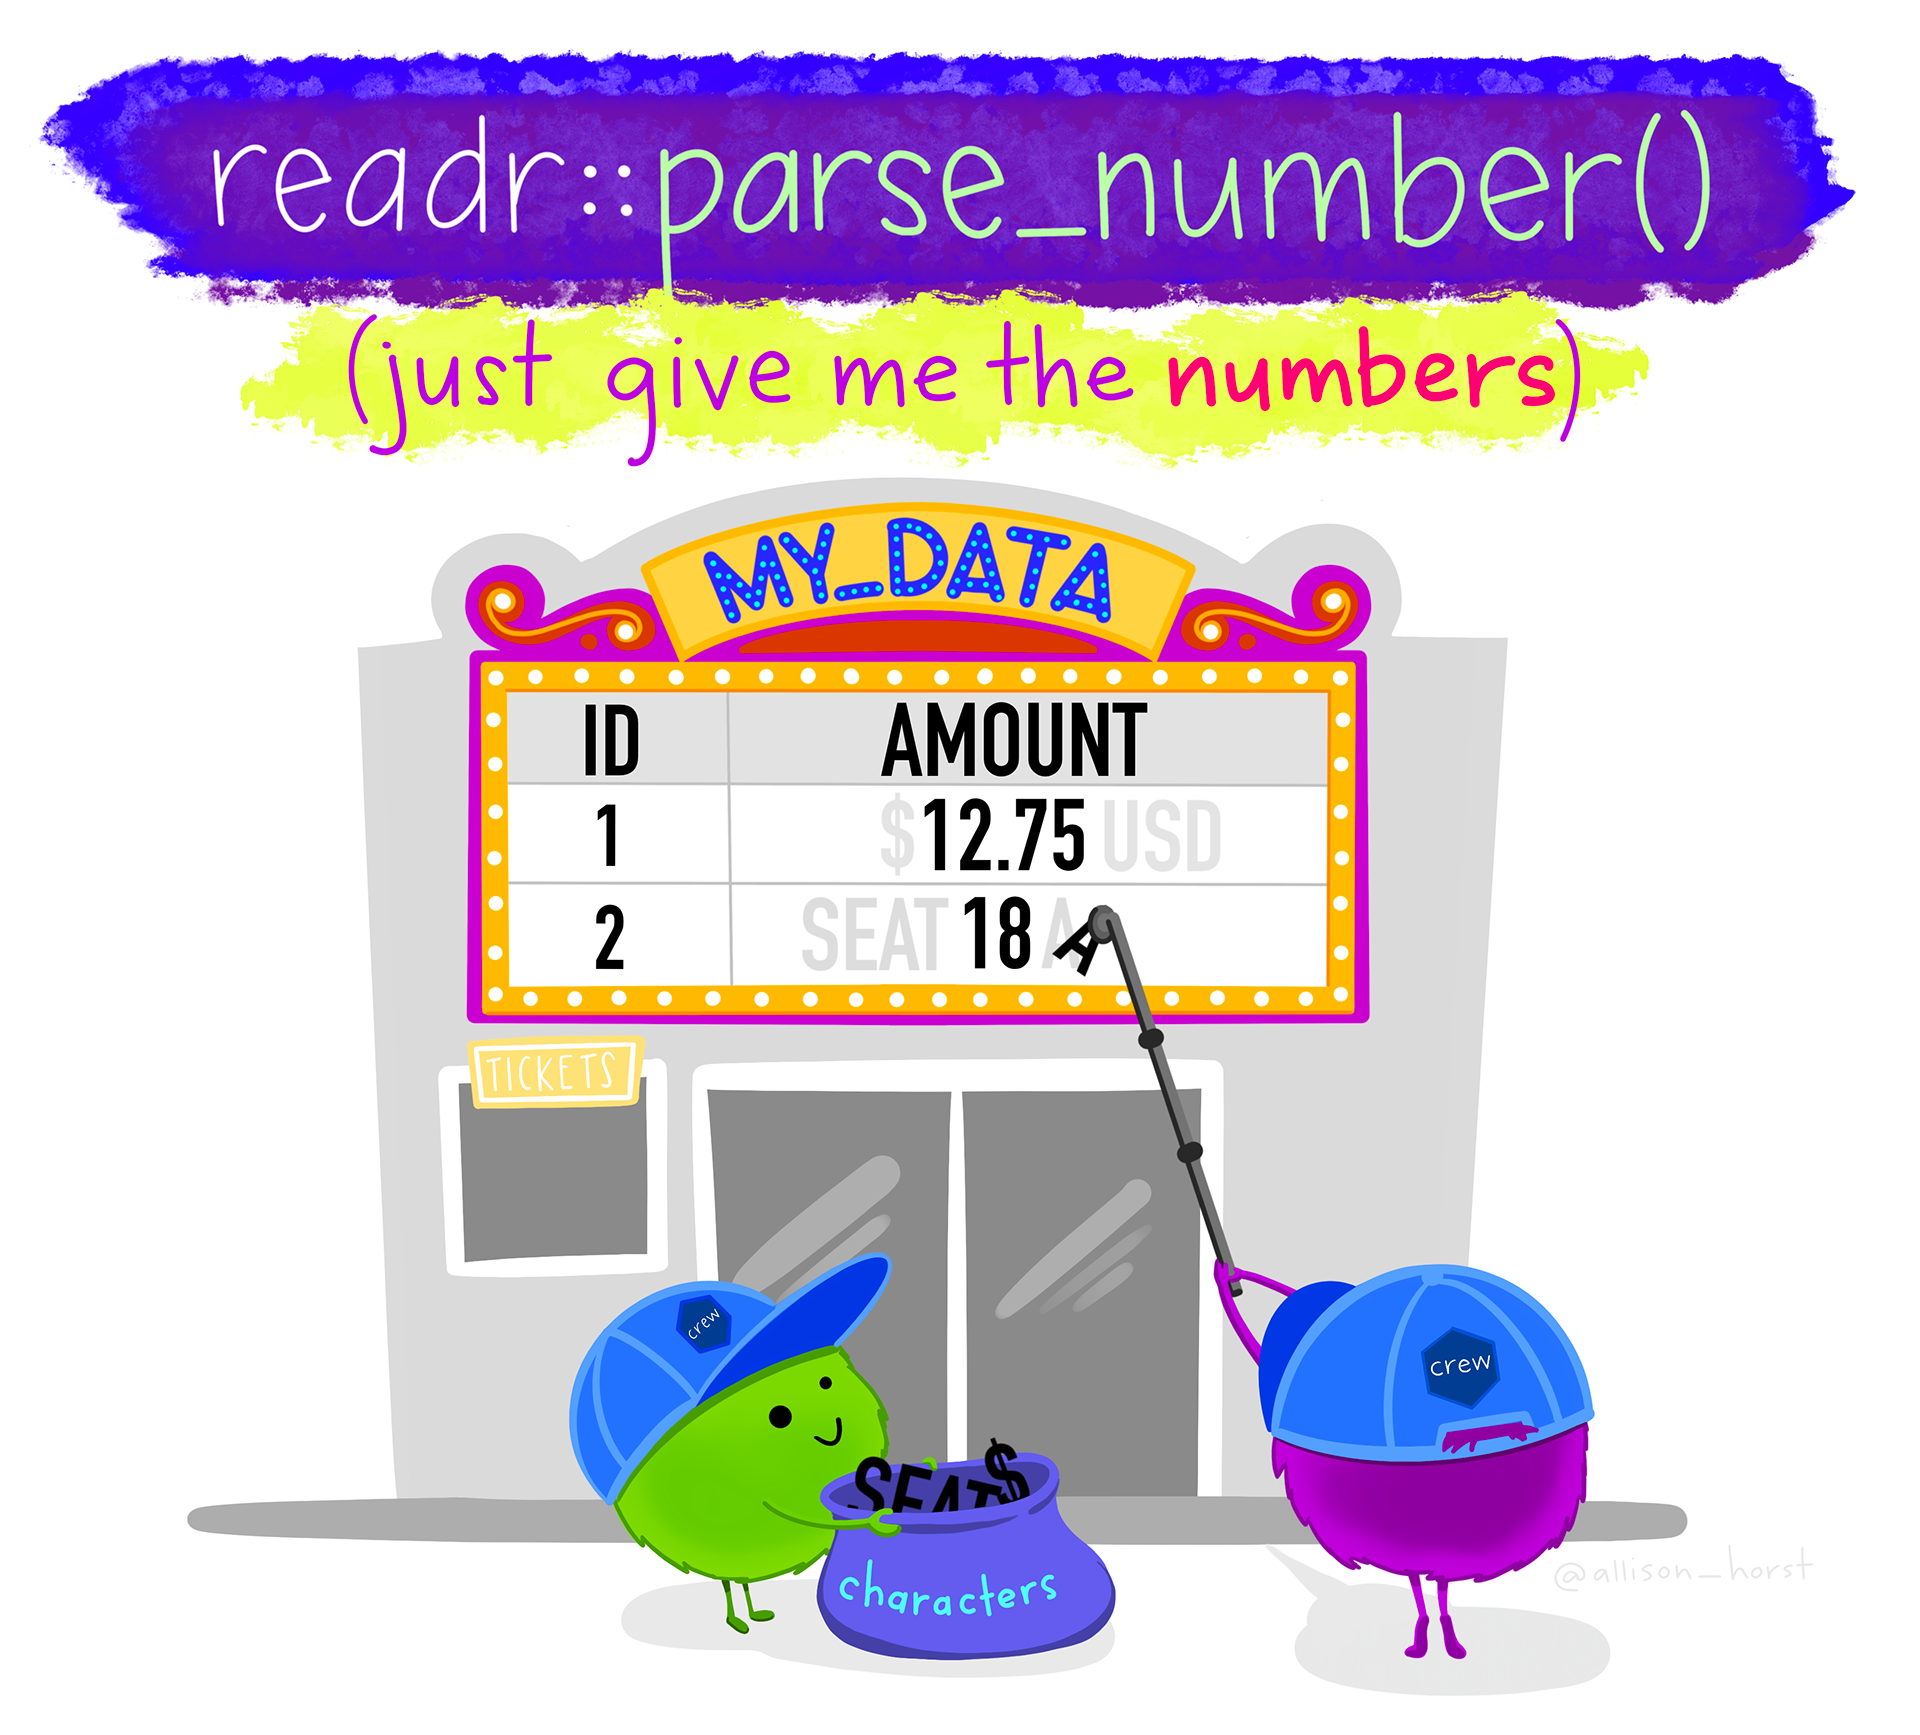
\includegraphics[width=0.5\textwidth,height=\textheight]{118_P_webscraping_text_files/mediabag/4fd04f07-7404-4371-8.png}

}

\caption{Artwork by @allisonhorst}

\end{figure}

\begin{Shaded}
\begin{Highlighting}[]
\CommentTok{\# runtime\_data \textless{}{-} URL \%\textgreater{}\%}
\CommentTok{\#   html\_nodes(".text{-}muted .runtime") \%\textgreater{}\%}
\CommentTok{\#   html\_text() \%\textgreater{}\%}
\CommentTok{\#   parse\_number() \%\textgreater{}\% \#this picks out only the numbers (and drops characters, in this case, "mins")}
\CommentTok{\#   as.numeric()}
\CommentTok{\# }
\CommentTok{\# runtime\_data}
\end{Highlighting}
\end{Shaded}

\hypertarget{ratings}{%
\subsection{Ratings}\label{ratings}}

Scrape IMBD for the ratings of the 50 most popular feature films in the
first 7 months of 2023.

Check out the relevant HTML code for Oppenheimer:

\begin{verbatim}
    <div class="inline-block ratings-imdb-rating" name="ir" data-value="8.6">
        <span class="global-sprite rating-star imdb-rating"></span>
        <strong>8.6</strong>
    </div>
\end{verbatim}

Let's scrape it!

\begin{Shaded}
\begin{Highlighting}[]
\CommentTok{\# rating\_data \textless{}{-} URL \%\textgreater{}\%}
\CommentTok{\#   html\_elements(".ratings{-}imdb{-}rating strong") \%\textgreater{}\%}
\CommentTok{\#   html\_text() \%\textgreater{}\%}
\CommentTok{\#   as.numeric()}
\CommentTok{\# }
\CommentTok{\# rating\_data}
\end{Highlighting}
\end{Shaded}

\begin{tcolorbox}[enhanced jigsaw, arc=.35mm, left=2mm, colbacktitle=quarto-callout-warning-color!10!white, coltitle=black, leftrule=.75mm, rightrule=.15mm, opacitybacktitle=0.6, titlerule=0mm, colframe=quarto-callout-warning-color-frame, toptitle=1mm, breakable, bottomtitle=1mm, bottomrule=.15mm, opacityback=0, title=\textcolor{quarto-callout-warning-color}{\faExclamationTriangle}\hspace{0.5em}{Warning}, toprule=.15mm, colback=white]

Notice that there are only 49 ratings listed, not 50! There is no way to
figure out which one is missing besides doing it by hand\ldots{}

Which one is it?

Once we figure out which one is it is, we should should add a blank
element for the rating for that movie using the \texttt{append}
function.

\texttt{rating\_data\ \textless{}-\ append(rating\_data,\ values=FALSE,\ after=11)}

\end{tcolorbox}

It's Killers of the Flower Moon (\#32)!

\begin{Shaded}
\begin{Highlighting}[]
\CommentTok{\#rating\_data \textless{}{-} append(rating\_data, values=NA, after=31)}
\end{Highlighting}
\end{Shaded}

Notice how it is the correct length (50) now!

\hypertarget{number-of-votes}{%
\subsection{Number of Votes}\label{number-of-votes}}

Scrape IMBD for the number of votes of the 50 most popular feature films
in the first 7 months of 2023.

Relevant code for Oppenheimer:

\begin{verbatim}
        <p class="sort-num_votes-visible">
                <span class="text-muted">Votes:</span>
                <span name="nv" data-value="391689">391,689</span>
        </p>
\end{verbatim}

Let's scrape it!

\begin{Shaded}
\begin{Highlighting}[]
\CommentTok{\# votes\_data \textless{}{-} URL \%\textgreater{}\%}
\CommentTok{\#   html\_elements(".sort{-}num\_votes{-}visible span:nth{-}child(2)") \%\textgreater{}\%}
\CommentTok{\#   html\_text() \%\textgreater{}\%}
\CommentTok{\#   parse\_number() \%\textgreater{}\%}
\CommentTok{\#   as.numeric()}
\CommentTok{\# }
\CommentTok{\# votes\_data}
\end{Highlighting}
\end{Shaded}

\begin{tcolorbox}[enhanced jigsaw, arc=.35mm, left=2mm, colbacktitle=quarto-callout-warning-color!10!white, coltitle=black, leftrule=.75mm, rightrule=.15mm, opacitybacktitle=0.6, titlerule=0mm, colframe=quarto-callout-warning-color-frame, toptitle=1mm, breakable, bottomtitle=1mm, bottomrule=.15mm, opacityback=0, title=\textcolor{quarto-callout-warning-color}{\faExclamationTriangle}\hspace{0.5em}{Warning}, toprule=.15mm, colback=white]

Same issue as before! We were supposed to have 50 but only got 49. It's
Killers of the Flower Moon (\#32), again!

\begin{Shaded}
\begin{Highlighting}[]
\CommentTok{\#votes\_data \textless{}{-} append(votes\_data, values=NA, after=31)}
\end{Highlighting}
\end{Shaded}

\end{tcolorbox}

\hypertarget{metascore}{%
\subsection{Metascore}\label{metascore}}

Scrape IMBD for the number of votes of the 50 most popular feature films
in the first 7 months of 2023.

Relevant code for Oppenheimer:

\begin{verbatim}
            <div class="inline-block ratings-metascore">
<span class="metascore  favorable">88        </span>
        Metascore
            </div>
\end{verbatim}

Let's scrape it!

\begin{Shaded}
\begin{Highlighting}[]
\CommentTok{\# metascore\_data \textless{}{-} URL \%\textgreater{}\%}
\CommentTok{\#   html\_elements(".metascore") \%\textgreater{}\%}
\CommentTok{\#   html\_text() \%\textgreater{}\%}
\CommentTok{\#   parse\_number() \%\textgreater{}\%}
\CommentTok{\#   as.numeric()}
\CommentTok{\# }
\CommentTok{\# metascore\_data}
\end{Highlighting}
\end{Shaded}

\begin{tcolorbox}[enhanced jigsaw, arc=.35mm, left=2mm, colbacktitle=quarto-callout-warning-color!10!white, coltitle=black, leftrule=.75mm, rightrule=.15mm, opacitybacktitle=0.6, titlerule=0mm, colframe=quarto-callout-warning-color-frame, toptitle=1mm, breakable, bottomtitle=1mm, bottomrule=.15mm, opacityback=0, title=\textcolor{quarto-callout-warning-color}{\faExclamationTriangle}\hspace{0.5em}{Warning}, toprule=.15mm, colback=white]

Yikes! Now we only have 41 when we should have 50.

We \emph{could} manually go through and figure out which 9 are missing
or we could reassess how important the metascore data is to us\ldots{}

\end{tcolorbox}

\hypertarget{combining-it-all-together-into-a-data-frame}{%
\section{Combining it all together into a data
frame!}\label{combining-it-all-together-into-a-data-frame}}

We can combine all this data into one data frame:

\begin{Shaded}
\begin{Highlighting}[]
\CommentTok{\# movies \textless{}{-} data.frame(Title = title\_data,}
\CommentTok{\# Runtime = runtime\_data,}
\CommentTok{\# Rating = rating\_data,}
\CommentTok{\# Votes = votes\_data}
\CommentTok{\# )}
\CommentTok{\# }
\CommentTok{\# movies}
\end{Highlighting}
\end{Shaded}

Make a list OR Make a plot!

\begin{Shaded}
\begin{Highlighting}[]
\CommentTok{\# ggplot(movies, aes(x=runtime\_data, y=rating\_data)) +}
\CommentTok{\#   geom\_point() +}
\CommentTok{\#   theme\_minimal() + }
\CommentTok{\#   xlab("Runtime (in minutes)") +}
\CommentTok{\#   ylab("IMDB Rating")}
\end{Highlighting}
\end{Shaded}




\end{document}
